%%% Local Variables: 
%%% mode: latex
%%% TeX-master: t
%%% End: 

\subsection{F4*: Building Most Restrictive Speed Profile and List of Targets i.r.t. the Train Front End} \label{ss:MRSPandListOfTargets}


The Statric Speed Profile (SSP) and speed restrictions in the “location based data” \FIXME{missing inputs to MRSP need to be added like Mode related speed restrictions} have to be combined to a most restrictive speed profile (MRSP) and list of targets for braking monitoring given as a distance from the LRBG. This is the task of the current function.

\subsubsection{Building of the MRSP}
The current function will combine the SSP and the list of speed restrictions (coming from TRS's, most restrictive braking distances, axle load profiles and level crossings \FIXME{missing inputs to MRSP need to be added like Mode related speed restrictions}) into a most restrictive speed profile (MRSP) and a list of targets subsequently used for braking curve monitoring.
Inputs: SSP and list of speed restrictions (including a mark which SR is not yet included in the MRSP and “list of targets”. \FIXME{missing inputs to MRSP need to be added like Mode related speed restrictions}
Outputs: MRSP and “list of targets for braking curve monitoring”, given as distances (one value without tolerance) from the front end of the train (taking into account the train length for speed increases if necessary).

The train specific static speed profile and the speed restrictions are used for:
\begin{itemize}
\item braking curve monitoring; according to the most restrictive targets
\item ceiling speed monitoring: according to the most restrictive speed at a certain location
\item release speed monitoring: according to the most restrictive speed at a certain location
\item indication monitoring: according to the most restrictive speed at a certain location
\item displaying the planning area to the driver; most restrictive speed profile in the area ahead.
\end{itemize}

For displaying to the driver (planning area) and guarding the actual ceiling- and release-speed, the maximum speed at any place shall be calculated (MRSP). For braking curve monitoring the actual most restrictive target is sufficient. The latter will not change till it's passed or revoked. Therefore a list of targets can be derived which has to guarded one by one, by braking curve monitoring.
In the modes FS (full supervision), OS (on sight) an LS (limited supervision) the MRSP can be derived from the SSP and speed restriction. In shunting and staff responsible (SH and SR) the mode profile can be given in the message commanding the transition to the state. 

In all cases the applicable most restrictive speed has to be respected. The restrictions can come from:
\begin{itemize}
\item Static Speed Profile (SSP)
\item Axle load Speed Profile (ASP)
\item Temporary Speed Restrictions (TSR)
\item Maximum Train Speed
\item Signalling related speed restriction (only level 1)
\item Mode related Speed Restriction.
\item STM Max speed
\item STM System speed
\item Level Crossing speed restriction (LX SR)
\item Override function related Speed Restriction
\item Speed restriction to ensure a given permitted braking distance 
\end{itemize}

\subsubsection{Usage of the MRSP}
The most restrictive speed profile is giving the lowest speed of the resulting SSP, and the list of speed restrictions.  When constructing the MRSP the distance to be taken into account that for speed decreases, is the minimum safe distance from the train front end (therefore the maximum “correction distance”) and for speed increases the maximum safe distance from the train front end (therefore the minimum “correction distance”).  The MRSP is to be used for supervising the actual speed and for displaying at the DMI (planning area). 

\subsubsection{Updating the MRSP}
\begin{itemize}
\item The MRSP has to be calculated every time a new SSP is received and when a new Last Relevant Balise Group (LRBG) is detected.
\item New speed restrictions can be included in the existing MRSP, without recalculating the complete MRSP. Therefore it's necessary to mark in the “list of speed restrictions” which speed restrictions have not yet been taken into account in the MRSP.
\item After every change of the train position (every cycle) the MRSP shall be updated according to the maximum and minimum distance driven (the maximum is relevant for speed decreases, the minimum is relevant for speed increases). This could lead to changing the order of points where the speed increases and points where the speed decreases.
\item the conditions for application of the single speed restriction has to be stored with the speed restriction and to be recalculated at least if one of the conditions change
\end{itemize}

An example is the case with two Temporary Speed Restrictions (TSRs) at a short distance:  

\begin{figure}[ht]
\centering
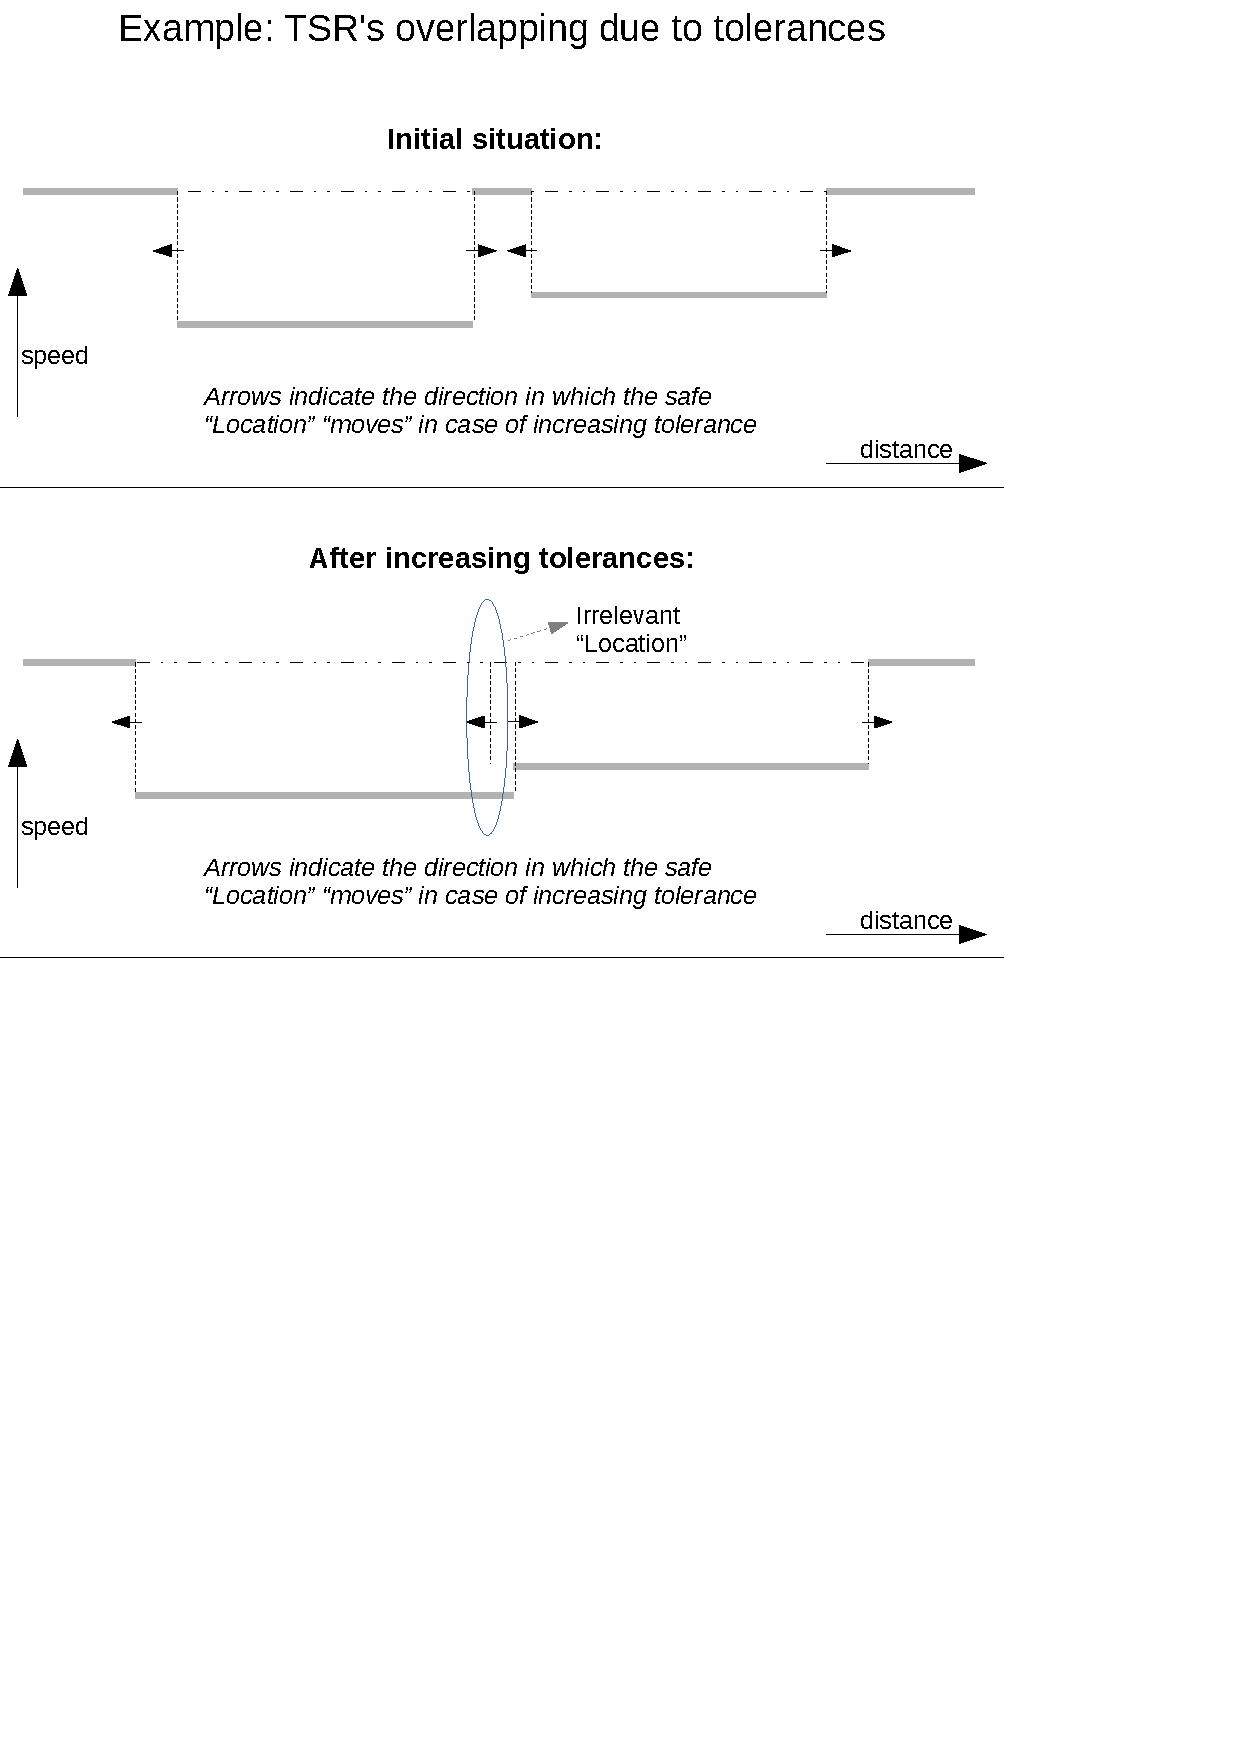
\includegraphics[trim = 0mm 130mm 0mm 0mm, scale=0.6]{../images/MRSPExample_TRSsOverlapping.pdf}
\caption{Example for overlapping TSRs due to increasing tolerances.}\label{fig:TSRoverlapping}
\end{figure}

The example of figure \ref{fig:TSRoverlapping} shows the effect of overlapping TSRs due to increasing tolerances. One point (distance from the train front end) shall be removed from the MRSP. 
\FIXME{further explanation on removing points from MRSP could be good here}

For braking curve monitoring (BCM) only speed decreases are relevant, and only those which do not lead to a higher “braking curve speed” than further targets with a lower target speed (see figure \ref{fig:ExampleListOfTargets}).

\subsubsection{Building the Most Restrictive Targets for BCM}
For braking curve monitoring the most restrictive target shall be known at every moment. In general a speed decrease in the MRSP is a potential target.  But not every speed decrease is a relevant target because they can be above the braking curve to another target ( see figure xxx). 


\begin{figure}[ht]
\centering
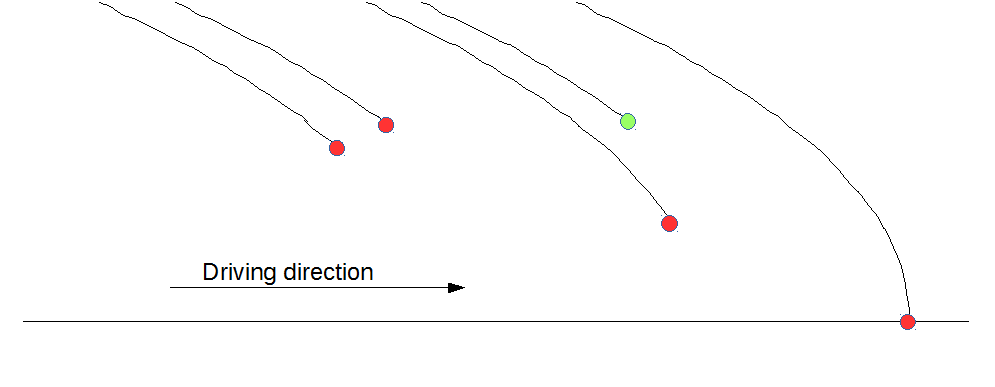
\includegraphics[scale=0.6]{../images/ExampleListOfMostRestrictiveTarget.png}
\caption{Example for ``list of most restrictive targets'' handled by braking curve monitoring.}\label{fig:ExampleListOfTargets}
\end{figure}


Figure \ref{fig:ExampleListOfTargets} shows examples of the selection of the “list of most restrictive targets” which have to be handled by “Braking Curve Monitoring” one by one. In the above example the “green” target will not be “most restrictive” and will thus not be relevant in the “list of most restrictive braking curve targets” unless the red target being more restrictive is revoked.

When analysing the MRSP from the furthest location towards the train front end, all relevant speed decreases (most restrictive targets for braking curve monitoring) are found. These locations will be stored (including the speed level) and have to be guarded one by one for braking curve monitoring.

\subsubsection{Updating the Targets for BCM}
The list of most restrictive targets shall be recalculated every time the MRSP has changed.

The data structure of the MRSP and list of target is different from the structure for general location based data because all locations are given as a distance from the LRBG only. So the data structure will not be based on the type “Location”.